\documentclass[aspectratio=169]{beamer}
\usepackage[utf8]{inputenc}
\usepackage{amsmath}
\usepackage{tikz}
\usepackage{pgfplots}
\usepackage{dsfont}
%\usepackage{opensans}
% \usepackage{fontspec}
% \setmainfont{Open Sans}

\usetikzlibrary {decorations.fractals,shadows,shapes.symbols,spy}
\AtBeginEnvironment{tikzpicture}{\tracinglostchars=0\relax}

\pgfplotsset{compat=1.18,samples=25}

\usetheme{NOVASBE}

\title[]{4509 - Bridging Mathematics}
\subtitle{Optimization}
\author{Paulo Fagandini}
\institute{}
\date{}

\newtheorem{defenition}{Definition}[section]
\newtheorem{proposition}{Conjecture}[section]

\begin{document}

\begin{frame}
    Let $f:\mathds{R}^n\rightarrow\mathds{R}$, and let $S\subseteq\mathds{R}^n$, the problem is:
    
    \begin{align*}
        \min_{x\in S} \quad f(x)
    \end{align*}
    
    Or finding $x^*\in S$ such that $$f(x^*)\leq f(x) \quad \forall x\in S$$
    
    \begin{definition}
        If $x\in S$, $x$ is said to be \textbf{feasible} for the optimization problem $\min_{x\in S}f(x)$.
    \end{definition}
    \vspace{0.5cm}
    \footnotesize{
    Note that to minimize $f(x)$ is equivalent to maximize $-f(x)$.}
\end{frame}

\begin{frame}
    \begin{definition}
        $x_0$ is a \textbf{local minimum} of $f$ in $S$ if, there is an open ball $B(x_0,r)$ such that for any $x\in B(x_0,r)\cap S$ it holds that $f(x_0)\leq f(x)$.
        
        \vspace{0.25cm}
        
        $x^*$ is a \textbf{global minimum} of $f$ in $S$ if for any $x\in S$ it holds that $f(x^*)\leq f(x)$.
    \end{definition}
    
    \begin{definition}
        Let the $\arg\min_{x\in S} f(x)$ represent the set of all global solutions to the problem of minimizing $f$ with $x\in S$.
    \end{definition}
    
    \vspace{0.5cm}
    
    \footnotesize{
    \textbf{Note}: For a maximization problem you have equivalently local maximum, global maximum, and $\arg\max_{x\in S} f(x)$.}
    
    
\end{frame}

\begin{frame}

\begin{proposition}
    Let $f:\mathds{R}^n\rightarrow\mathds{R}$ be a continuous function. Let $S\in\mathds{R}^n$ be compact. Then the problem
    \begin{align*}
        \max_{x\in S} f(x)
    \end{align*}
    has at least one solution, or equivalently $\arg\min_{x\in S}f(x)\neq\emptyset$.
\end{proposition}

\begin{proposition}
    If $S_1\subseteq S_2$, then $min(f,S_1)\geq min(f,S_2)$.
\end{proposition}
    
\end{frame}

\begin{frame}
    
    Prove the first one, 10 min.
    
    \begin{proof}
    \begin{itemize}
        \item $f$ is continuous in $S$, and $S$ is compact, so $f(S)$ is compact.\pause
        \item $f(S)$ compact means it is bounded, and furthermore closed, so the supremum (lowest upper bound) is in the set.\pause
        \item $\exists s\in S$ such that $f(s)=\sup f(S)$.\pause
    \end{itemize}
    
    Maybe it can be shown with contradiction, choosing an $x$, then see if it is the maximizer, done, if it is not, it is because you know of another that gives you a higher value in $f(x)$, so you move to that one. Then you can build a sequence, which you now it has a subsequence that converges in $S$ ($S$ is compact), and therefore the limit must be the maximizer, and therefore $f(x_n)$ converges to the maximum of the function as well.
    
    \end{proof}
    
\end{frame}

\begin{frame}
    Now the second one 5 min.\pause
    
    \begin{proof}
        
        Trivial. By contradiction. Let $s_1 \in S \leq s_2 \in S$. As $s_i\in S_1 \Rightarrow s_1\in S_2$, because $S_1\subseteq S_2$, then $s_2$ cannot be a minimizer.
        
    \end{proof}
    
\end{frame}

\begin{frame}
    
    These are the necessary conditions for optimality for the unconstrained problem $(S=\mathds{R}^n)$, when $f$ is at least twice differentiable:
    
    \begin{proposition}
    $x_0$ is a local optimum of $f:\mathds{R}^n\rightarrow\mathds{R}$ if:
    \begin{enumerate}
        \item First Order Condition:  $\nabla f(x_0)=0$.
        \item Second Order Conditions:
        \begin{enumerate}
            \item $H(f,x_0)\geq 0$ (Hessian positive semi definite) then $x_0$ is a local minimum.
        \item $H(f,x_0)\leq 0$ (Hessian negative semi definite) then $x_0$ is a local maximum.  
        \end{enumerate}
    \end{enumerate}
    \end{proposition}
    
\end{frame}

\begin{frame}{Example}
    Let $f(x,y)=x^2+y^2$,
    
    \begin{enumerate}
        \item FOC: $\frac{\partial f}{\partial x}(x^*)=0$ and $\frac{\partial f}{\partial y}(x^*)=0$
        \begin{enumerate}
            \item $f_{x}=2x$, so $f_{x}=0 \Rightarrow x^*=0$
            \item $f_{y}=2y$, so $f_{y}=0 \Rightarrow y^*=0$
        \end{enumerate}
        \item SOC:
        \begin{enumerate}
            \item Hessian: $$\mathcal{H}=\begin{pmatrix}\frac{\partial^2 f}{\partial x^2} & \frac{\partial^2 f}{\partial x\partial y} \\ \frac{\partial^2 f}{\partial y\partial x} & \frac{\partial^2 f}{\partial y^2}\end{pmatrix}=\begin{pmatrix}2&0\\0&2\end{pmatrix}$$
            \item $\det(\mathcal{H}-\lambda I) = (2-\lambda)^2$, so $\det(\mathcal{H}-\lambda I)=0$ $\Rightarrow$ $\lambda=2$
            \item All $e.v.$ are strictly positive, so $\mathcal{H}$ is positive definite.
            \item Finally $(0,0)$ is a minimum.
        \end{enumerate}
    \end{enumerate}
    
\end{frame}

\begin{frame}{Example}
    \begin{columns}
        \begin{column}{0.47\textwidth}
            \begin{center}
                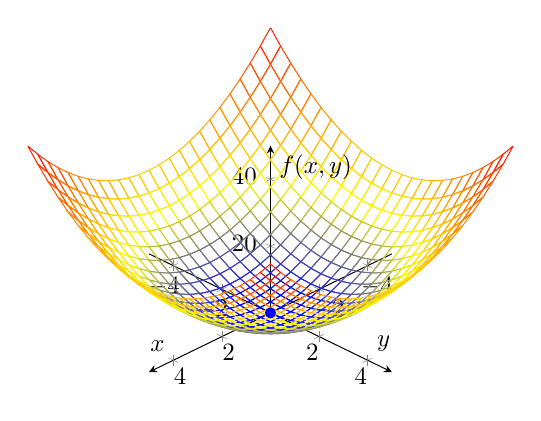
\begin{tikzpicture}[scale=0.9]
                    \begin{axis}[view={135}{45},
                                grid=major,
                                xlabel=$x$,
                                ylabel=$y$,
                                zlabel={$f(x,y)$},
                                axis lines=center]
                        \addplot3[mesh] {x^2+y^2};
                        \addplot3[only marks,mark=*,color=blue] coordinates { (0,0,0) };

                    \end{axis}
                \end{tikzpicture}
            \end{center}
        \end{column}
        
        \pause
        
        \begin{column}{0.47\textwidth}
            \begin{center}
                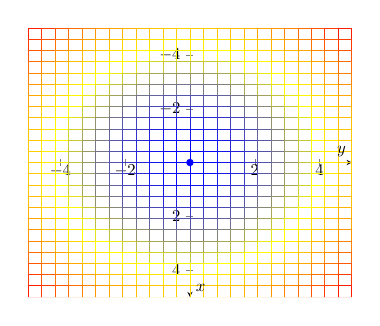
\begin{tikzpicture}[scale=0.6]
                    \begin{axis}[view={90}{90},
                                grid=major,
                                xlabel=$x$,
                                ylabel=$y$,
                                zlabel={$f(x,y)$},
                                axis lines=center]
                        \addplot3[mesh] {x^2+y^2};
                        \addplot3[only marks,mark=*,color=blue] coordinates { (0,0,0) };
                    \end{axis}
                \end{tikzpicture}
            \end{center}
        \end{column}
    \end{columns}
\end{frame}

\begin{frame}{Example}
    Let $f(x,y)=x^2-y^2$,
    
    \begin{enumerate}
        \item FOC: $\frac{\partial f}{\partial x}(x^*)=0$ and $\frac{\partial f}{\partial y}(x^*)=0$
        \begin{enumerate}
            \item $f_{x}=2x$, so $f_{x}=0 \Rightarrow x^*=0$
            \item $f_{y}=-2y$, so $f_{y}=0 \Rightarrow y^*=0$
        \end{enumerate}
        \item SOC:
        \begin{enumerate}
            \item Hessian: $$\mathcal{H}=\begin{pmatrix}\frac{\partial^2 f}{\partial x^2} & \frac{\partial^2 f}{\partial x\partial y} \\ \frac{\partial^2 f}{\partial y\partial x} & \frac{\partial^2 f}{\partial y^2}\end{pmatrix}=\begin{pmatrix}2&0\\0&-2\end{pmatrix}$$
            \item $\det(\mathcal{H}-\lambda I) = -(4-\lambda^2)$, so $\det(\mathcal{H}-\lambda I)=0$ $\Rightarrow$ $\lambda=\pm2$
            \item The $e.v.$s are not strictly positive or negative, so we cannot say anything about the positiveness of $\mathcal{H}$.
            \item Finally we cannot say that $(0,0)$ is a minimum or a maximum.
        \end{enumerate}
    \end{enumerate}

\end{frame}

\begin{frame}{Example}
    \begin{columns}
        \begin{column}{0.47\textwidth}
            \begin{center}
                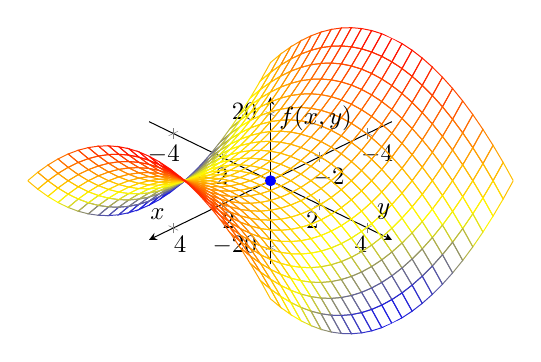
\begin{tikzpicture}[scale=0.9]
                    \begin{axis}[view={135}{45},
                                grid=major,
                                xlabel=$x$,
                                ylabel=$y$,
                                zlabel={$f(x,y)$},
                                axis lines=center]
                        \addplot3[mesh] {x^2-y^2};
                        \addplot3[only marks,mark=*,color=blue] coordinates { (0,0,0) };

                    \end{axis}
                \end{tikzpicture}
            \end{center}
        \end{column}
        
        \pause
        
        \begin{column}{0.47\textwidth}
            \begin{center}
                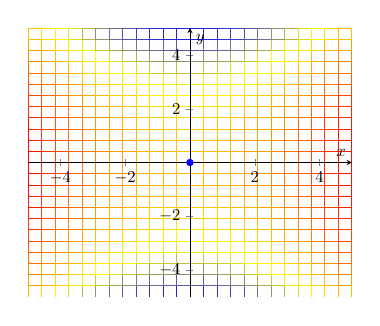
\begin{tikzpicture}[scale=0.6]
                    \begin{axis}[view={0}{90},
                                grid=major,
                                xlabel=$x$,
                                ylabel=$y$,
                                zlabel={$f(x,y)$},
                                axis lines=center]
                        \addplot3[mesh] {x^2-y^2};
                        \addplot3[only marks,mark=*,color=blue] coordinates { (0,0,0) };
                    \end{axis}
                \end{tikzpicture}
            \end{center}
        \end{column}
    \end{columns}
\end{frame}


\begin{frame}{Equality Constraints}

    Consider now the constrained problem, and assume that $S\subseteq\mathds{R}^n$ can be described as a set of equations that $x\in\mathds{R}^n$ must satisfy, say $h_i(x)=0$.
    
    $$S=\{x\in\mathds{R}^n|h_i(x)=0,\quad i=1,...,m\}$$
    The problem is now
    \begin{align*}
        \min_{x\in\mathds{R}^n}\quad &f(x)\\
        s.t.\quad &h_i(x)=0,\quad i=1,...,m
    \end{align*}


From now on, to simplify notation, we will use $\min_x$ instead of $\min_{x\in\mathds{R}^n}$.
\end{frame}

\begin{frame}
    \begin{definition}[Mangasarian-Fromowitz constraint qualification]
        The feasible point $x^*\in\mathds{R}^n$ is said to be \textbf{regular} if the set of gradients $\nabla h_i(x^*)$ for $i=1,...,m$ is l.i.
    \end{definition}
    
    \vspace{0.5cm}
    
    If this is not satisfied, the solution you find might not be an optimum.
\end{frame}

\begin{frame}
    \begin{definition}
    
    Let $f:\mathds{R}^n\rightarrow\mathds{R}$, continuous and differentiable.
    
    Consider the following optimization problem:
    
    \begin{align*}
        \min_{x}\quad &f(x)\\
        s.t.\quad & h_i(x)=0,\quad i=1,...,n
    \end{align*}
    
    Define the function $\mathcal{L}:\mathds{R}^n\times\mathds{R}^m\rightarrow\mathds{R}$ such that:
    
    $$\mathcal{L}(x_1,\ldots,x_n,\lambda_1,\dots,\lambda_m)=f(x)+\sum_{i=1}^{m}\lambda_i h_i(x)$$
    
    $\mathcal{L}$ is called the  \textbf{Lagrangian}, and $\lambda_i$ for $i=1,...,m$ are called the \textbf{Lagrange multipliers}.
    
    \end{definition}
\end{frame}

\begin{frame}
\begin{theorem}
    Let $x^*$ to be a local minimum of $f$, such that $h_i(x^*)=0$ for $i=1,...,m$. Also let $x^*$ be regular. Then, there is a vector $\lambda=(\lambda_1,\dots,\lambda_m)^t\in\mathds{R}^m$ such that:
    
    \begin{align*}
        \frac{\partial f(x^*)}{\partial x_i}+\sum_{j=1}^m\lambda_j \frac{\partial h_j(x^*)}{\partial x_i} =0, \quad i=1,\ldots,n\\
        \frac{\partial f(x^*)}{\partial \lambda_j}=0,\quad j=1,...,m
    \end{align*}
\end{theorem}
\end{frame}

\begin{frame}
    \begin{theorem}[Second Order Conditions]
        Let $x^*$ be a local minimum for $f$, satisfying $h_j(x^*)=0$ for every $j=1,...,m$. Assume further that $x^*$ is regular. Consider $\lambda\in\mathds{R}^m$ the vector of Lagrange multipliers of the problem, then the matrix
        
        \begin{align*}
            \mathcal{H}=H(f,x^*)+\sum_{j=1}^m\lambda_j H(h_j,x^*)
        \end{align*}
        
        is positive semi definite in the set $M:=\{y\in\mathds{R}^n|\nabla h_j(x^*)\cdot y=0,\forall j=1,...,m\}$
        
        
    \end{theorem}
\end{frame}

\begin{frame}{Example}
    Let $f(x,y)=x^2y$. Maximize $f(x,y)$ such that $x^2+y^2=1$.
\end{frame}

\begin{frame}{Example}
    \begin{columns}
        \begin{column}{0.47\textwidth}
            \begin{center}
                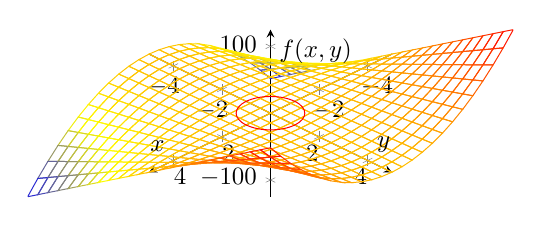
\begin{tikzpicture}[scale=0.9]
                    \begin{axis}[view={135}{45},
                                grid=major,
                                xlabel=$x$,
                                ylabel=$y$,
                                zlabel={$f(x,y)$},
                                axis lines=center]
                        \addplot3[mesh] {x^2*y};
                        \draw[color=red] (axis cs:0,0,0) circle (1);
                    \end{axis}
                \end{tikzpicture}
            \end{center}
        \end{column}
        
        \pause
        
        \begin{column}{0.47\textwidth}
            \begin{center}
                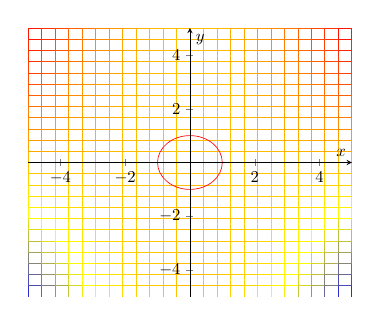
\begin{tikzpicture}[scale=0.6]
                    \begin{axis}[view={0}{90},
                                grid=major,
                                xlabel=$x$,
                                ylabel=$y$,
                                zlabel={$f(x,y)$},
                                axis lines=center]
                        \addplot3[mesh] {x^2*y};
                        \draw[color=red] (axis cs:0,0,0) circle (1);
                    \end{axis}
                \end{tikzpicture}
            \end{center}
        \end{column}
    \end{columns}
\end{frame}

\begin{frame}{Example}
    \begin{center}
        \begin{tikzpicture}[scale=1]
            \begin{axis}[view={0}{90},
                        grid=none,
                        xlabel=$x$,
                        ylabel=$y$,
                        zlabel={$f(x,y)$},
                        axis lines=center,
                        domain=-2:2,
                        ticks=none]
                        opacity=0,
            
                \addplot3[opacity=1,contour gnuplot={levels={-1.5,-1,-0.5,-0.25,0.25,0.5,1,1.5},labels={false}},thick] {x^2*y};
                
                %\addplot3[opacity=0,contour gnuplot={levels={0.3849},labels={false}},thick] {x^2*y};
            
                \addplot3[opacity=0.5,blue,-stealth,samples=15,quiver={u={2*x*y},v={x^2},scale arrows=0.03,}] {x^2*y};
            
                %\addplot3[opacity=0,contour gnuplot={levels={0.1,0.5,1,1.5},labels={false}},thick] {x^2+y^2};
                
                %\addplot3[opacity=0,red,-stealth,samples=15,quiver={u={2*x},v={2*y},scale arrows=0.03,}] {x^2+y^2};
            
                %\addplot3[opacity=0,contour gnuplot={levels={1},labels={false}},thick] {x^2+y^2};
        
            \end{axis}
        \end{tikzpicture}
    \end{center}
\end{frame}

\begin{frame}{Example}
    \begin{center}
        \begin{tikzpicture}[scale=1]
            \begin{axis}[view={0}{90},
                        grid=none,
                        xlabel=$x$,
                        ylabel=$y$,
                        zlabel={$f(x,y)$},
                        axis lines=center,
                        domain=-2:2,
                        ticks=none]
                    
                %\addplot3[opacity=0,contour gnuplot={levels={-1.5,-1,-0.5,-0.25,0.25,0.5,1,1.5},labels={false}},thick] {x^2*y};
                
                %\addplot3[opacity=0,contour gnuplot={levels={0.3849},labels={false}},thick] {x^2*y};
            
                %\addplot3[opacity=0,blue,-stealth,samples=15,quiver={u={2*x*y},v={x^2},scale arrows=0.03,}] {x^2*y};
            
                \addplot3[opacity=1,contour gnuplot={levels={0.1,0.5,1,1.5},labels={false}},thick] {x^2+y^2};
                
                \addplot3[opacity=0.5,red,-stealth,samples=10,quiver={u={2*x},v={2*y},scale arrows=0.03,}] {x^2+y^2};
            
                %\addplot3[opacity=0,contour gnuplot={levels={1},labels={false}},thick] {x^2+y^2};
        
            \end{axis}
        \end{tikzpicture}
    \end{center}
\end{frame}

\begin{frame}{Example}
    \begin{center}
        \begin{tikzpicture}[scale=1]
        
            \begin{axis}[view={0}{90},
                        grid=none,
                        xlabel=$x$,
                        ylabel=$y$,
                        zlabel={$f(x,y)$},
                        axis lines=center,
                        domain=-2:2,
                        ticks=none]
            
                %\addplot3[opacity=0,contour gnuplot={levels={-1.5,-1,-0.5,-0.25,0.25,0.5,1,1.5},labels={false}},thick] {x^2*y};
                
                \addplot3[opacity=1,contour gnuplot={levels={0.3849},labels={false}},thick] {x^2*y};
            
                \addplot3[opacity=0.3,blue,-stealth,samples=10,quiver={u={2*x*y},v={x^2},scale arrows=0.03,}] {x^2*y};
            
                %\addplot3[opacity=0,contour gnuplot={levels={0.1,0.5,1,1.5},labels={false}},thick] {x^2+y^2};
                
                \addplot3[opacity=0.3,red,-stealth,samples=10,quiver={u={2*x},v={2*y},scale arrows=0.03,}] {x^2+y^2};
            
                \addplot3[opacity=1,contour gnuplot={levels={1},labels={false}},thick] {x^2+y^2};
                
            \end{axis}
            
        \end{tikzpicture}
    \end{center}
\end{frame}

\begin{frame}{Example}
    \begin{center}
        \begin{tikzpicture}[scale=1]
        
            \begin{axis}[view={0}{90},
                        grid=none,
                        xlabel=$x$,
                        ylabel=$y$,
                        zlabel={$f(x,y)$},
                        axis lines=center,
                        domain=0.75:1,
                        y domain = 0.4:0.65,
                        ticks=none]
            
                \addplot3[opacity=1,blue,contour gnuplot={levels={0.3849},labels={false}},thick] {x^2*y};
                \addplot3[opacity=0.5,blue,-stealth,samples=5,quiver={u={2*x*y},v={x^2},scale arrows=0.03,},thick] {x^2*y};
            
                \addplot3[opacity=1,red,contour gnuplot={levels={1},labels={false}},thick] {x^2+y^2};
                \addplot3[opacity=0.5,red,-stealth,samples=5,quiver={u={2*x},v={2*y},scale arrows=0.03,},thick] {x^2+y^2};
                
            \end{axis}
            
        \end{tikzpicture}
    \end{center}
\end{frame}

\begin{frame}{Example}
    The Lagrangian is:
    \begin{align*}
        \mathcal{L}=x^2y+\lambda (x^2+y^2-1)
    \end{align*}
\end{frame}

\begin{frame}{Inequality Constraints}

    Assume now that $S\subseteq\mathds{R}^n$ can be described as a set of equations and inequalities that $x\in\mathds{R}^n$ must satisfy, say $h_i(x)=0$ and $g_j(x)\leq0$.
    
    \footnotesize{
    $$S=\{x\in\mathds{R}^n|h_i(x)=0, i=1,...,m\}\cap\{x\in\mathds{R}^n|g_j(x)\leq 0, j=1,...,p\}$$}
    
    \normalsize
    
    The problem is now
    \begin{align*}
        \min_{x}\quad &f(x)\\
        s.t.\quad &h_i(x)=0,\quad i=1,...,m\\
        &g_j(x)\leq 0,\quad j=1,...,p
    \end{align*}

\end{frame}

\begin{frame}
    \begin{definition}
    
        Let $x^*\in\mathds{R}^n$ be such that $h_i(x^*)=0, i=1,...,m$ and $g_j(x^*)\leq 0,j=1,...,p$. $x^*$ is called \textbf{regular} for the constraints if the set of gradients
        
        $$\{\nabla h_i(x^*),\nabla g_j(x^*), i=1,...,m,\quad j=\in J_A\}$$
        
        is $l.i.$, where $J_A\subseteq\{1,...,p\}$ represents the active constraints in $x^*$.
    
    \end{definition}
\end{frame}


\begin{frame}
    \begin{definition}
        Let $x^*$ be a solution to the problem in the previous slide. The inequality constraint $g_k(x^*)$ is called \textbf{active}, if $g_k(x^*)=0$. Otherwise it is considered \textbf{slack}.
    \end{definition}
    
    \vspace{0.5cm}
    
    If you knew ex-ante which constraints are active, you can use the Lagrange method to find the solution.
\end{frame}

\begin{frame}
    \begin{theorem}[Karush-Kuhn-Tucker]
        Let $x^*$ be a local minimum for the problem:
        \begin{align*}
            \min_x \quad &f(x)\\
            s.t.\quad & h_i(x)=0,i=1,\ldots,m\\
            &g_j(x)\leq 0, j=1,\ldots,p
        \end{align*}
        
        Such that $x^*$ is regular for the constraints, then there are multipliers $\lambda_i,i=1,...,m$ and $\mu_j,j=1,...,p$ such that:
        
        \begin{enumerate}
            \item $\mu_j\geq 0$ for $j=1,...,p$.
            \item $\nabla f(x^*)+\sum_{i=1}^m\lambda_i\nabla h_i(x^*)+\sum_{j=1}^p\mu_j\nabla g_j(x^*)=0$.
            \item $\sum_{j=1}^p \mu_j g_j(x^*)=0$
        \end{enumerate}
    \end{theorem}
\end{frame}

\begin{frame}
    \begin{theorem}[Second Order Conditions]
        Let $x^*$ be a local minimum of $f$ that satisfies $h_i(x^*)=0,i=1,\ldots,m$, $g_j(x^*)\leq0,j=1,\dots,p$. Assume further than $x^*$ is regular for the constraints. Then the matrix
        \begin{align*}
        \mathcal{H}=H(f,x^*)+\sum_{i=1}^m \lambda_i H(h_i,x^*)+\sum_{j=1}^p \mu_j H(g_j,x^*)
        \end{align*}
        
        Is positive semi definite in the set that is orthogonal to the active constraints:
        
        $M:=\{y\in\mathds{R}^n|\nabla h_j(x^*)\cdot y=0,\forall j=1,...,m\}\cap\{y\in\mathds{R}^n|\nabla g_k(x^*)\cdot y=0, k\in J_A\}$
        
    \end{theorem}
\end{frame}

\begin{frame}
    \begin{theorem}[Envelope's Theorem]
        Consider the following optimization problem,
        \begin{align*}
            \min_x \quad &f(x,\alpha)\\
            s.t.\quad &h_j(x,\alpha)=0, j=1,...,m
        \end{align*}
        
        Where $\alpha=(\alpha_1,...,\alpha_l)\in\mathds{R}^l$ are parameters of the problem. Consider further that all the functions ($f$, $h$s) are continuously differentiable. Let $x(\alpha)$ a solution and $min(f)(\alpha)=f(x(\alpha),\alpha)$ the minimum value taken by $f$. Then, $\forall k=1,...,l$ holds that:
        
        \begin{align*}
            \frac{d \min(f)(\alpha)}{d \alpha_k}=\frac{\partial f(x(\alpha),\alpha)}{\partial \alpha_k}+\sum_{j=1}^m\lambda_j\frac{\partial h_j(x(\alpha),\alpha)}{\partial \alpha_k}
        \end{align*}
        Where $\lambda_j$ is the multiplier of the optimality conditions.
    \end{theorem}
\end{frame}

\begin{frame}
    \begin{theorem}[Berge's Maximum]
        Consider the following optimization problem
        \begin{align*}
            \max_x\quad &f(x,\alpha)\\
            s.t.\quad &g_j(x,\alpha)\leq 0,j=1,...,p
        \end{align*}
        
        Assume that for $\alpha^*$, the solution is $x^*=x(\alpha^*)$. Then, if $f$ and the $g$s are continuous in $(x^*,\alpha^*)$, and the set defined by the inequality constraints is compact, then the function $\max(f)(\alpha)=f(x^*(\alpha),\alpha)$ is continuous in $\alpha^*$. Furthermore, if the solution $x^*(\alpha)$ is unique, then, $x^*(\alpha)$ is also continuous.
        
    \end{theorem}
\end{frame}

\end{document}
